Let $(X, \rho)$ be a metric space. Let $\B$ be the family of bounded sets in $X$.

\begin{definition}\label{def:totally_bounded_set}
  The space $A \subseteq X$ is called \uline{totally bounded} if any of the following equivalent conditions hold:

  \begin{defenum}
    \item\label{def:totally_bounded_set/sets} For every $\varepsilon > 0$ there exists a finite cover of $A$ with sets with diameter at most $\varepsilon$.
    \item\label{def:totally_bounded_set/balls} For every $\varepsilon > 0$ there exists a finite cover of $A$ with balls of radius $\varepsilon$.
    \item\label{def:totally_bounded_set/zero_noncompactness/sets} Kuratowski's noncompactness measure (see~\cref{def:noncompactness_measures/sets}) $\alpha(A)$ is zero.
    \item\label{def:totally_bounded_set/zero_noncompactness/balls} The ball noncompactness measure (see~\cref{def:noncompactness_measures/balls}) $\beta(A)$ is zero.
    \item\label{def:totally_bounded_set/fundamental_subsequences} Every sequence in $A$ admits a fundamental subsequence.
  \end{defenum}

  Totally bounded sets are sometimes called \uline{precompact} (see \cref{def:compact_sets}) because of~\cref{thm:metric_sequentially_compact_iff_compact}. This equivalence requires the metric space to be complete, however.
\end{definition}
\begin{proof}
  The equivalences \ref{def:totally_bounded_set/sets} $\iff$ \ref{def:totally_bounded_set/zero_noncompactness/sets} and \ref{def:totally_bounded_set/balls} $\iff$ \ref{def:totally_bounded_set/zero_noncompactness/balls} are straightforward.

  (\ref{def:totally_bounded_set/balls} $\implies$ \ref{def:totally_bounded_set/sets}) Given $\varepsilon > 0$, any cover of $A$ with balls of radius $\frac \varepsilon 2$ is a cover with sets of diameter $\varepsilon$.

  (\ref{def:totally_bounded_set/sets} $\implies$ \ref{def:totally_bounded_set/balls}) Fix $\varepsilon > 0$ and $\mu \in (0, \varepsilon)$ and let $A_1, \ldots, A_n \subseteq \PS X$ be a finite cover of $A$ with sets of diameter at most $\mu$.

  Choose\AOC~a point $x_k$ from every $A_k$, $k = 1, \ldots, n$. We then have that for every $k = 1, \ldots, n$,
  \begin{align*}
    A_k \subseteq \Cl B(x_k, \mu) \subsetneq B(x_k, \varepsilon)
    \\
    \implies A \subseteq \bigcup_{k=1}^n A_k \subseteq \bigcup_{k=1}^n B(x_k, \mu) \subsetneq \bigcup_{k=1}^n B(x_k, \varepsilon),
  \end{align*}
  hence $x_1, \ldots, x_n$ are centers of $\varepsilon$-balls that cover $A$.

  (\ref{def:totally_bounded_set/balls} $\implies$ \ref{def:totally_bounded_set/fundamental_subsequences}) Let $\{ x_n \} \subseteq A$ be any sequence.

  If we assume\LEM\ that $\{ x_n \}$ has no fundamental subsequence, then there exists $\varepsilon_0 > 0$ such that $\rho(x_k, x_m) > \varepsilon_0$ for any $n, m \in \ZPos$.

  Consider a finite cover of $A$ with $\varepsilon_0$-balls. By the pigeonhole principle, at least one of the balls contains more than one element of the sequence, which contradicts the assumption that all elements of the sequence have a distance of at least $\varepsilon_0$.

  Hence an arbitrary sequence in $A$ has a fundamental subsequence.

  (\ref{def:totally_bounded_set/fundamental_subsequences} $\implies$ \ref{def:totally_bounded_set/balls}) Assume\LEM\ that there exists $\varepsilon_0 > 0$, such that $A$ admits no finite cover by $\varepsilon_0$-balls.

  Define $x_1 \in X, x_2 \in X \setminus B(x_1, \varepsilon_0), \ldots$, so that every two elements of the sequence $\{ x_n \}$ have a distance of at least $\varepsilon_0$. But then the sequence is does not admit a fundamental subsequence, which contradicts our assumption.

  This contradiction proves that $A$ admits a finite cover by $\varepsilon$-balls for every $\varepsilon > 0$.
\end{proof}

\begin{corollary}\label{thm:metric_compact_iff_closed_totally_bounded}
  Assume that $X$ is complete. The set $A \subseteq X$ is sequentially compact if and only if it is closed and totally bounded.
\end{corollary}
\begin{proof}
  The property that every sequence has a fundamental subsequence is equivalent to sequential compactness for a closed set in a complete metric space.
\end{proof}

\begin{proposition}\label{thm:closure_of_totally_bounded_is_totally_bounded}
  If a set $A \subseteq X$ is totally bounded, then so is its closure $\Cl A$.
\end{proposition}
\begin{proof}
  Let $\varepsilon > 0$ and $\mu \in (0, \varepsilon)$ and let $x_1, \ldots, x_n \in X$ be the centers of a cover of $A$ with $\mu$-balls.

  If $y$ is a point in $\Cl A \setminus A$, there exists a point $z \in A$ with $\rho(y, z) < \varepsilon - \mu$. Let $x_k \in A$ be one of the centers whose $\mu$-balls contain $z$. We then have that $y \in B(x_k, \varepsilon)$ since
  \begin{align*}
    \rho(x_k, z) \leq \rho(x_k, y) + \rho(y, z) < \mu + \varepsilon - \mu = \varepsilon.
  \end{align*}

  Hence the balls $\Cl B(x_k, \varepsilon)$ cover $\Cl A$, i.e.
  \begin{align*}
    \Cl A \subseteq \bigcup_{k=1}^n B(x_k, \varepsilon).
  \end{align*}
\end{proof}

\begin{lemma}[Lebesgue's covering lemma]\label{thm:lebesgue_covering_lemma}
  Assume that $X$ is complete. Let $A \subseteq X$ be sequentially compact. Given an open cover $\F \subseteq \PS A$, there exists a number $\delta > 0$ such that every $\delta$-ball with a center in $A$ is contained in some set of the cover $\F$.
\end{lemma}
\begin{proof}
  Assume\LEM\ that no such number $\delta > 0$ exists. Then for any natural number $n \in \ZPos$, there exists an element $x_n \in A$ such that the ball $B(x_n, \frac 1 n)$ is not contained in any set of the cover $\F$. Since $A$ is sequentially compact, the sequence $\{ x_n \}_n$ contains a convergent subsequence $\{ x_{n_k} \}_k$.

  Define
  \begin{align*}
    x \coloneqq \lim_{k \to \infty} x_{n_k}.
  \end{align*}

  Let\AOC\ $E$ be a set in $\F$ that contains $x$. Since $E$ is open, there exists some radius $r > 0$ such that $B(x, r) \subseteq E$.

  Choose any $k_0 > \frac 2 r$ such that $\rho(x_{n_{k_0}}, x) < \frac r 2$. By the triangle inequality,
  \begin{align*}
    B \left(x_{n_k}, \frac 1 k \right) \subsetneq B \left(x_k, \frac r 2 \right) \subseteq B(x, r) \subseteq E,
  \end{align*}
  which contradicts the choice of the sequence $\{ x_n \}_n$.

  Hence there exists a $\delta > 0$ such that for every $x \in A$, the ball $B(x, \delta)$ is contained in some element $E$ of the cover $\F$.
\end{proof}

\begin{theorem}\label{thm:metric_compact_iff_sequentially_compact}
  Assume that $X$ is complete. The set $A \subseteq X$ is compact if and only if it is sequentially compact
\end{theorem}
\begin{proof}
  ($\implies$) Let $\F \subseteq \PS X$ be an open cover of $A$.

  By the Lebesgue covering lemma (\cref{thm:lebesgue_covering_lemma}), there exists $\delta > 0$ such that for every $x \in A$, the ball $B(x, \delta)$ is contained in some set of the cover $\F$. Let $x_1, \ldots, x_n$ be a cover of $A$ with $\delta$-balls.

  For each $k = 1, \ldots, n$ we have that the ball $B(x_k, \delta)$ is contained in some set $E_k \in \F$. Hence $E_1, \ldots, E_n$ is a finite subcover of $A$, because
  \begin{align*}
    A \subseteq \bigcup_{k=1}^\infty B(x_k, \delta) \subseteq \bigcup_{k=1}^\infty E_k.
  \end{align*}

  Thus $A$ is compact.

  ($\impliedby$) Let $A$ be compact. Fix $\varepsilon > 0$ and take the cover
  \begin{align*}
    \F \coloneqq \{ B(a, \varepsilon) \colon a \in A \}.
  \end{align*}

  By compactness of $A$, there exists a finite subcover. Thus a finite cover of $A$ with $\varepsilon$-balls exists for every $\varepsilon > 0$. \Cref{def:totally_bounded_set} then implies that total boundedness is equivalent to sequential compactness because $X$ is complete and $A$ is closed.
\end{proof}

\begin{definition}\label{def:noncompactness_measures}(\cite[definition 7.1]{Deimling1985})
  We define the following functions
  \begin{defenum}
    \item\label{def:noncompactness_measures/sets} The \uline{Kuratowski measure of noncompactness},
    \begin{align*}
      &\alpha: \B \to \RPos \\
      &\alpha(A) \coloneqq \inf \{d > 0 \colon \exists U_1, \ldots, U_n \subseteq X: \Diam {U_k} < d \land A \subseteq \cup_{k=1}^n U_k \}
    \end{align*}

    \item\label{def:noncompactness_measures/balls} The \uline{ball measure of noncompactness},
    \begin{align*}
      &\beta: \B \to \RPos \\
      &\beta(A) \coloneqq \inf \{r > 0 \colon \exists x_1, \ldots, x_2 \in X: A \subseteq \cup_{k=1}^n B(x_k, r) \}
    \end{align*}
  \end{defenum}
\end{definition}

\begin{example}\label{ex:noncompactness_measures}(\cite[exercise 7.3]{Deimling1985})
  Consider the subsets $A_2 \subseteq A_3 \subseteq A_1 \subseteq C([0, 1])$, defined by
  \begin{align*}
    A_1 \coloneqq \left\{
      x \in C([0, 1]) \colon \begin{aligned}
        0 \leq t \leq 1 \implies 0 \leq x(t) \leq 1 \\
        x(0) = 0, x(1) = 1 \\
      \end{aligned}
    \right\}
    \\
    A_2 \coloneqq \left\{
      x \in A_1 \colon \begin{aligned}
        0 \leq t \leq \frac 1 2 \implies 0 \leq x(t) \leq \frac 1 2 \\
        \frac 1 2 \leq t \leq 1 \implies \frac 1 2 \leq x(t) \leq 1
      \end{aligned}
    \right\}
    \\
    A_3 \coloneqq \left\{
      x \in A_1 \colon \begin{aligned}
        0 \leq t \leq \frac 1 2 \implies 0 \leq x(t) \leq \frac 2 3 \\
        \frac 1 2 \leq t \leq 1 \implies \frac 1 3 \leq x(t) \leq 1
      \end{aligned}
    \right\}
  \end{align*}

  Then $\alpha(A_1) = 1, \alpha(A_2) = \frac 1 2, \alpha(A_3) = \frac 1 3$ and $\beta(A_1) = \beta(A_2) = \beta(A_3) = \frac 1 2$.
\end{example}
\begin{proof}
  Since the distance between any two functions from $B_1$ is at most 1, we have that $\Diam B_1 = 1$ and $\alpha(B_1) \leq 1$.

  Fix $\varepsilon > 0$. For any function $f \in B_1$, continuity of $f$ gives us a radius $\delta_f > 0$ such that
  \begin{align*}
    x < 2 \delta_f \implies f(x) < \varepsilon.
  \end{align*}

  \begin{figure}[h]
    \begin{center}
      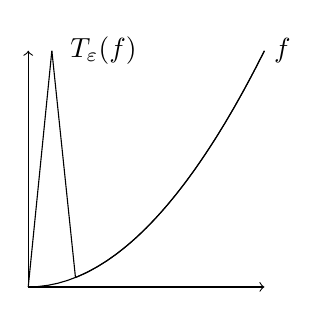
\begin{tikzpicture}[scale=3]
        \draw[->] (0, 0) -- (1, 0);
        \draw[->] (0, 0) -- (0, 1);

        \draw[domain=0:1, variable=\x] plot ({\x}, {\x^2}) node[right] {$f$};

        \draw (1/2, 1) node[left] {$T_\varepsilon(f)$};
        \draw[domain=0:0.1, variable=\x] plot ({\x}, {10 * \x});
        \draw[domain=0.1:0.2, variable=\x] plot ({\x}, {0.04 + (1 - 0.04) * (2 - 10 * \x)});
        \draw[domain=0.2:1, variable=\x] plot ({\x}, {\x^2});
      \end{tikzpicture}
    \end{center}
  \end{figure}

  Define
  \begin{align*}
    T_\varepsilon(f)(x) \coloneqq \begin{cases}
      \frac x \delta_f, &0 \leq x < \delta_f \\
      f(\delta_f) + [1 - f(\delta_f)] (2 - \frac x {\delta_f}), &\delta_f \leq x < 2 \delta_f \\
      f(x), &x \geq 2 \delta_f,
    \end{cases}
  \end{align*}
  so that
  \begin{align*}
    \Norm{T_\varepsilon(f) - f}
    \geq
    T_\varepsilon(f) (\delta_f) - f(\delta_f)
    =
    1 - f(\delta_f)
    >
    1 - \varepsilon.
  \end{align*}

  Additionally, because $\delta_{T_\varepsilon(f)} < \delta_f$, we have that $f(\delta_{T_\varepsilon(f)}) < \varepsilon$ and
  \begin{align*}
    \Norm{T_\varepsilon(T_\varepsilon(f)) - f}
    \geq
    T_\varepsilon(T_\varepsilon(f)) (\delta_{T_\varepsilon(f)}) - f(\delta_{T_\varepsilon(f)})
    =
    1 - f(\delta_{T_\varepsilon(f)})
    >
    1 - \varepsilon.
  \end{align*}

  Given any function $f$, we can construct a sequence $\{ f, T_\varepsilon(f), T_\varepsilon(T_\varepsilon(f)), \ldots \}$ such that any two elements of the sequence have a distance of at least $1 - \varepsilon$ between them, hence $B_1$ cannot be covered by a finite $(1-\varepsilon)$-net and $\alpha(B_1) \geq 1 - \varepsilon$. Since $\varepsilon > 0$ can be made arbitrarily small, this implies that $\alpha(B_1) \geq 1$.

  Hence we have $\alpha(B_1) = 1$.

  In the set $B_2$, the maximum distance between two functions is $\frac 1 2$, thus $\Diam(B_2) = \frac 1 2$ and $\alpha(B_2) \leq \frac 1 2$. We can then define an operator similar to $T_\varepsilon$ that creates \enquote{spikes} of height $\frac 1 2$ to prove the reverse inequality, obtaining
  \begin{align*}
    \alpha(B_2) = \frac 1 2.
  \end{align*}

  Finally, the set $B_3$ has diameter $\frac 2 3$ and hence $\alpha(B_3) = \frac 2 3$.

  The ball measure for $B_1$ satisfies the inequalities
  \begin{align*}
    \frac 1 2 \leq \beta(B_1) \leq 1.
  \end{align*}

  Additionally, $B_1$ is strictly contained in the ball centered in the constant function $\frac 1 2$ with radius $\frac 1 2$, which implies that $\beta(B_1) \leq \frac 1 2$, hence $\beta(B_1) = \frac 1 2$.

  For $B_2$ we have
  \begin{align*}
    \frac 1 4 \leq \beta(B_2) \leq \frac 1 2.
  \end{align*}

  Assume that for some $\mu \in \left(\frac 1 4, \frac 1 2 \right)$ the set $B_2$ can be covered by a finite $\mu$-net and let $\{ f_1, \ldots, f_n \} \subsetneq C([0, 1])$ be the centers of the balls of this cover.

  Denote by $y \in \left[0, \frac 1 2 \right)$ the largest value for which any of the functions $f_1, \ldots, f_n$ attains $\frac 1 2$ and, if none of them attains $\frac 1 2$ in the interval $\left[0, \frac 1 2 \right)$, define $y = 0$.

  Define $z$ analogously as the smallest such value in the interval $\left(\frac 1 2, 1 \right]$ and let $z = 1$ if none of the functions attains $\frac 1 2$ in the interval.

  Define $g$ by
  \begin{align*}
    g(x) \coloneqq \begin{cases}
      0, &0 \leq x \leq y, \\
      \frac{x - y} {1 - 2y}, &y < x \leq \frac 1 2, \\
      \frac{x + z - 1} {2z - 1}, &\frac 1 2 < x < z, \\
      1, &z \leq x \leq 1.
    \end{cases}
  \end{align*}

  \begin{figure}[h]
    \begin{center}
      \begin{tikzpicture}[scale=3]
        \draw[->] (0, 0) -- (1, 0);
        \draw[->] (0, 0) -- (0, 1);

        \draw[domain=1/3:1/2, variable=\x] plot ({\x}, {3 * \x - 1}) node[left] {$g$};
        \draw (1/3, -1/9) node {$y$};
        \draw[domain=1/2:3/4, variable=\x] plot ({\x}, {2 * \x - 1/2});
        \draw (3/4, 1) node[left] {$z$};
        \draw[domain=3/4:1, variable=\x] plot ({\x}, 1);
      \end{tikzpicture}
    \end{center}
  \end{figure}

  We then have that $g \in B_2$ and $\Norm{g - f_k} \geq \frac 1 2$ for all $f_k$, hence $B_2$ cannot be covered by balls with centers $f_1, \ldots, f_n$ and radius $\mu < \frac 1 2$. Thus $\beta(B_2) \geq \frac 1 2$.

  For the ball measures, because of the inclusion $B_2 \subsetneq B_3 \subsetneq B_1$, we have
  \begin{align*}
    \frac 1 2 = \beta(B_2) \leq \beta(B_3) \leq \beta(B_1) = \frac 1 2,
  \end{align*}
  hence $\beta(B_3) = \frac 1 2$.
\end{proof}

\begin{theorem}\label{thm:noncompact_cantor_theorem}(\cite[exercise 7.4]{Deimling1985}, Cantor's theorem for noncompact sets)
  Let $X$ be a Banach space and $\{ A_n \}_n$ be a decreasing sequence of nonempty closed subsets such that $\alpha(A_n) \to 0$. Then $A \coloneqq \bigcap_n A_n$ is nonempty and compact.
\end{theorem}
\begin{proof}
  The set $A$ is compact because it is closed as the intersection of closed sets and $\alpha(A) \leq \alpha(A_n) \to 0$, hence $\alpha(A) = 0$.

  It remains to show that $A$ is nonempty.
  Choose\AOC\ any sequence $\{ x_n \}_n$ where $x_n \in A_n$. Since any finite set is compact, we have that for any $k \geq 1$
  \begin{align*}
    \alpha(\{ x_n \}_{n \geq 1})
    =
    \max\{ \alpha(\{ x_n \}_{n < k}), \alpha(\{ x_n \}_{n \geq k}) \}
    =
    \alpha(\{ x_n \}_{n \geq k})
    \leq
    \alpha(A_k) \to 0,
  \end{align*}
  hence the set $\{ x_n \colon n \geq 1 \}$ is compact and thus sequentially compact. We can choose a convergent subsequence $\{ x_{n_k} \}_k$ of $\{ x_n \}_n$ whose limit lies in every $A_n$ (since they are closed) and, consequently, in their intersection $A$. So $A$ is nonempty.
\end{proof}
